%# -*- coding: utf-8-unix -*-
%%==================================================
%% chapter01.tex for SJTU Master Thesis
%%==================================================

\chapter{绪论}
\label{chap:intro}



\section{研究背景和意义}
\label{sec:background}

船舶在无限深广的静水中直线航行产生的波系最早由开尔文给出
\supercite{Thomson1887ship}。
根据开尔文的分析,船后的波系被限制在一个与航迹夹角$-\psi^K\le\psi\le\psi^K$的楔形
区域中,角$\psi^K\approx19^\circ28'$称为开尔文角。在该楔形区域内每一点都存在两种波,
即横波和散波。从开尔文的分析中还可看出,由横波和散波组成的波系其波形与船长$L$或船型
都无关,只取决于航速$V$。因此,开尔文波系与弗洛德数$F\equiv V/\sqrt{gL}$无关,
且对于任何船型---不论是单体船、双体船、潜艇,还是气垫船等---都是相同的。
具体来说,开尔文波系决定于无因次化的坐标$(X,Y)g/V^2$,其中$g$是重力加速度。
图\ref{fig:kelvinwake}显示了开尔文波系。
许多观测和数值计算结果表明,常见的排水型船舶其船行波与开尔文波系非常相似,
且波系中波高最大的波位于$\psi=\pm\psi^K$的射线上,这也和开尔文的分析一致。

\begin{figure}[htp]
  \centering
  \captionstyle{\centering}
  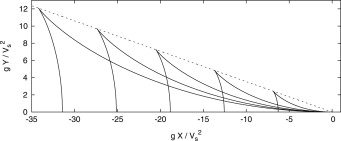
\includegraphics[width=0.5\textwidth]{chap1/kelvinwake.jpg}
  \bicaption[fig:kelvinwake]{开尔文波系}{在无限深广的静水中直线航行的船舶产生的开尔文波系,由横波和散波组成}{Fig}{The classical Kelvin pattern of 
    transverse and divergent waves created by a ship that advances at constant speed in calm water of large depth}
\end{figure}

然而大量由安装在卫星上的高分辨率合成孔径雷达(Synthetic-apeture radar, SAR)
拍摄的船行波照片显示,
船行波中最明显的波位于$\psi=\pm\psi_{\max}$的射线上,其中$\psi_{\max}$显著小于开尔文
角$\psi^K$\supercite{Taylor1910Resistance,Baker1915Ship,Munk1987Ships,Brown1989Observations,Reed2002Ship,Fang2011Kelvin,Rabaud2013Ship}。
这些窄V字形尾迹在图中呈现明亮的边缘,表明边缘的雷达后向散射 (radar backscatter) 
增强,而窄V字形内部呈现暗色,表明雷达后向散射较弱\supercite{Reed2002Ship}。
这里将$\psi_{\max}$称为主要兴波角(dominant wake angle)。
特别地,\parencite{Rabaud2013Ship}报告了37例不同船舶在不同航速下的主要兴波角
$\psi_{\max}$数据,其弗洛德数$F$分布于$0.1<F<1.7$。其中处于$0.6<F$的12个观测数据显示
,主要兴波角$\psi_{\max}$一致并显著地小于开尔文角$\psi^K$,且主要兴波角$\psi_{\max}$
随弗洛德数$F$的增大而减小。而处于$0.1<F<0.6$区域的主要兴波角$\psi_{\max}$大致位于开
尔文角$\psi^K$附近。
图\ref{fig:rabaudobserv}显示了\parencite{Rabaud2013Ship}的观测结果。

\begin{figure}[htp]
  \centering
  \captionstyle{\centering}
  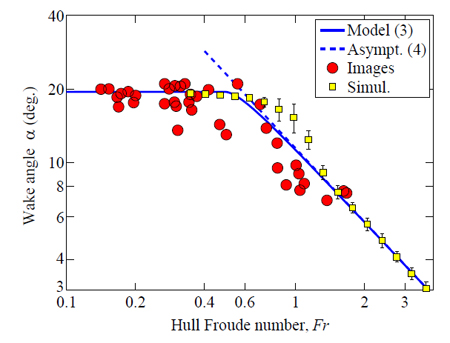
\includegraphics[width=0.5\textwidth]{chap1/expRM.jpg}
  \bicaption[fig:rabaudobserv]{观测的主要兴波角$\psi_{\max}$与弗洛德数$F$的关系}
  {由\parencite{Rabaud2013Ship}观测的37艘船的主要兴波角$\psi_{\max}$与弗洛德数$F$
的关系}{Fig}{Relation between the dominant wake angles $\psi_{\max}$ and the Froude 
numbers $F$ of 37 observed narrow V-shaped ship wakes}
\end{figure}

众所周知,开尔文的经典分析\supercite{Thomson1887ship}是水波理论的基础,几乎出现在
任何一本介绍水波和水动力学的书籍中,如
\parencite{newman1977marine,sheng2003principle}。
而观测到主要兴波角$\psi_{\max}$显著小于开尔文角$\psi_{\max}$的现象表面上与开尔文的
理论相悖。因此解释这一现象十分具有重要的理论意义。

船体阻力按产生阻力的原因来分类,则船体总阻力$R_t$由兴波阻力$R_w$、摩擦阻力$R_f$和
粘压阻力$R_{pv}$三者组成:$R_t=R_w+R_f+R_{pv}$。
船行波是产生兴波阻力的原因\supercite{Michell1898wave,Wehausen1973Wave},
而兴波阻力是船舶阻力的重要组成部分,特别是对高速船,兴波阻力占总阻力的40\%-50\%。
根据弗洛德定律,对于给定船型,船体兴波阻力系数$C_w$仅仅是弗洛德数$F$的函数。
对于较丰满船,兴波阻力系数$c_w$随弗洛德数$F$的增加快速增加,而当$F\approx0.4$时,
船首波的波长约等于船长$\Lambda\approx L$,此时船就像深陷在首波波峰后的槽中一样,因此
兴波阻力系数急剧增加。与该弗洛德数对应的航速称为船身极速 (hull speed)。
滑行 (planing) 是克服船身极速的方式之一,但是很多现代排水型船无需滑行即可轻易克服
船身极速。随着$F$的增大,$C_w$继续增大,瘦削船在$F=0.5$附近存在$C_w$峰值区,
当$F>0.5$时,$C_w$随$F$的增大而减小。窄V字形尾迹的夹角---即主要兴波角$\psi_{\max}$
---随弗洛德数$F$减小的现象与兴波阻力系数$C_w$随弗洛德数$F$的增大而减小的现象
之间的相似性暗示窄V字形尾迹与兴波阻力之间存在联系\supercite{Rabaud2014narrow}。
\parencite{Rabaud2014narrow}还注意到
$\psi_{\max}$随$F$的增大而减小的临界弗洛德数与$C_w$开始减小的临界弗洛德数的数值
相差不大。因此研究这一问题也有助于增加对兴波阻力的认识,从而为减小船舶阻力、
提高船舶快速性提供新的视角。

SAR图像中经常出现船舶尾迹,通过分析这些尾迹可以获得关于船舶的信息。
因此SAR图像是得到实用的船舶数据的重要来源。
由此获得的数据可以与基于船舶自我报告的船舶自动识别系统
(Automatic Identification System, AIS) 中的数据进行对比验证。
除了用来验证AIS系统中的数据,这些信息还可能被用来对海域进行广域监视
(wide area surveillance)。现代SAR传感器在短时间内就能产生大量数据,
这对自动舰船尾迹检测 (automatic ship wake detection) 产生了需求
\supercite{Crisp2004state}。
对窄V字形尾迹的理解关乎能否从SAR图像中得到关于船舶的有用信息
\supercite{Tunaley2009narrow}。

\section{国内外发展现状}
\label{sec:statofart}

\subsection{窄V字形船行波的理论分析}
针对主要兴波角$\psi_{\max}$显著小于开尔文角$\psi^K$的现象,许多研究者给出了解释。
\parencite{Brown1989Observations}将主要兴波角$\psi_{\max}$处的波与非线性孤立波的特征
进行了对比,并认为主要兴波角$\psi_{\max}$的产生可能是因为该处非线性孤立波的存在。
\parencite{Mei1991Note}认为由周围环境的波浪造成的船舶运动可能是产生该非线性孤立波的
原因。\parencite{Zhu2008Resonant}的研究显示了船行波与环境波浪的三阶共振干涉会在
开尔文波系内产生新的波。此波所处的角度与船舶航速和波浪参数有关。
而\parencite{Shugan2006Kelvin}的研究表明,环境波浪的存在本身就会改变开尔文波系
的楔形夹角。如果船舶航向与波浪传播方向一致,楔形区域的夹角将会变小。
\parencite{Fang2011Kelvin}考虑了风和有限水深对开尔文波系的影响。
在水深弗洛德数$F_h>1$时,开尔文角随$F_h$的增大而减小。
虽然开尔文的分析中未考虑到的因素---非线性、船舶摇荡运动、环境波浪、风、有限水深---
会显著地影响开尔文波系,这并不表示观测的主要兴波角$\psi_{\max}$
小于开尔文角的现象是由于这些因素引起的。

\parencite{Rabaud2013Ship}在线性水波理论的基础上,引入了下列假设:
船舶兴波的波长不能超过船长。因此,一旦兴波的波速达到与波长等于船长对应的波速后
便无法增加。他们的分析表明,当弗洛德数$F>0.5$时主要兴波角$\psi_{\max}$
的大小与$F$成反比。\parencite{Moisy2014Mach}与\parencite{Moisy2014Scaling}
又将上述假设应用到非轴对称形的自由面压力分布的兴波与考虑表面张力的情况下,
也得到类似结论。虽然\parencite{Rabaud2013Ship}得出的解析关系$\psi_{\max}(F)$
与该文中的观测结果相对一致,然而文中并未就其引入的假设提供任何解释。
众所周知,在线性水波理论的框架下,开尔文波系中波长最大的波传播方向为船舶的航向,
其(无因次)波长为$\lambda^{\max}\equiv\Lambda^{\max}/L=2\pi F^2$,
因此当弗洛德数$F>0.4$时,波长大于船长。
可见\parencite{Rabaud2013Ship}中的假设是违背线性水波理论的。
因此如果没有其他证据支持该假设,很难使人信服。事实上,\parencite{He2015Comparison}
论证了在线性水波理论的框架下,波长不超过某截断波长$\lambda<\lambda^{cut}=1$的假设
在数学上与兴波角度不超过某截断兴波角$\psi<\psi^{cut}$是完全等价的。具体来说,
\begin{equation}
  \lambda\le\lambda^{cut}
  \label{eq:rabaudassump}
\end{equation}
等价于
\begin{equation}
  \psi\le\psi^{cut}\equiv\tan^{-1}\left(
  \frac{\sqrt{\lambda^{\max}/\lambda^{cut}-1}}{2\lambda^{\max}/\lambda^{cut}-1}
  \right)
  \label{eq:wavlencut}
\end{equation}
所以限制了波长不能超过船长,自然也就限制了兴波角不能超过某个角度。
因此,\parencite{Rabaud2013Ship}的解释存在逻辑错误。

\parencite{Darmon2014Kelvin}考虑了高斯分布的压力场的自由面兴波,从理论分析中证明了
波幅最大的波所处的射线其角度按$F^{-1}$的形式减小。\parencite{Darmon2014Kelvin}的结果
暗示SAR观测到的主要兴波角$\psi_{\max}$很可能就是波幅最大的波所处的射线的角度。
相比其他解释,其优美之处在于首次从波幅的大小解释窄V字形船行波的出现\supercite{Dias2014Ship}。
\parencite{Darmon2014Kelvin}的结果也表明了即使不考虑非线性、船舶摇荡运动、环境波浪、
风、有限水深等这些外部因素,只用线性势流理论也能产生窄V字形船行波。
\parencite{Benzaquen2014Wake}将\parencite{Darmon2014Kelvin}的结果推广到各向异性
的自由面压力分布形式,并得到相似结论。在\parencite{Darmon2014Kelvin}对主要兴波角
$\psi_{\max}$理解的基础上,\parencite{Pethiyagoda2014What}和\parencite{Pethiyagoda2015Wake}
研究了非线性和有限水深效应对主要兴波角$\psi_{\max}$的影响,\parencite{Ellingsen2014Ship}
研究了剪切流对主要兴波角$\psi_{\max}$的影响。当弗洛德数$F\gg1$时,主要兴波角
$\psi_{\max}$随弗洛德数$F$的变化规律几乎不受剪切流的影响。
虽然\parencite{Darmon2014Kelvin}展示了主要兴波角也即波幅最大的波所对应的角
$\psi_{\max}$随弗洛德数$F$的增大而减小的关系,但其并未解释出现这种现象的原因。


需要指出的是,不同的船舶在船长、航速、船型上有很大差别,它们产生的船行波也大不相同。
比如说,全部浸入水中的潜艇或低速排水型船(如油轮)产生的波系主要包括横波,
而高速艇产生的波系中散波占主导。事实上,船行波的波形很大程度上受弗洛德数$F$和
船体表面形状的影响。这并不与开尔文的结论矛盾。开尔文基于驻相点法
(method of stationary phase) 的渐近分析只考虑波的相位,没有也不能考虑横波和散波的
波幅。而横波和散波的波幅在被开尔文角包括的船后楔形区域内变化,
且很大程度上受弗洛德数$F$和船体表面形状的影响。这是产生多种多样的船行波的原因。

回顾开尔文的压力点兴波理论,开尔文波系实际上是开尔文根据流体力学理论求得的一个压力点
在水面上作匀速直线运动时的波形图。而船行波正是由于船舶在水面上航行时船体周围流体压力
变化引起的。最大压力区产生于船体首尾驻点附近,其兴波作用最强,因此这两个最大压力区的
兴波可以简化为两个压力点兴波的叠加。考虑两个压力点的兴波也意味着引入了新的物理量:
长度。因此考虑船舶首尾波系之间的干涉成为可能。事实上,船舶工程师通常利用首尾横波的
干涉选择船长,力求避免波阻峰点,设法处于波阻谷点\supercite{sheng2003principle}。
然而首尾散波的干涉并未引起人们的重视。

\parencite{Noblesse2014Why}首先从波浪干涉的角度解释窄V字形船行波的出现。
\parencite{Noblesse2014Why}证明了主要兴波角$\psi_{\max}$处波幅最大是由高航速时
散波的相长干涉效应 (constructive interference) 造成的。众所周知,在线性势流理论的
框架下,船体的兴波速度势可以表示成在船体表面上分布的点源兴波速度势的叠加\supercite{Noblesse2011Practical,Noblesse2013Neumann}。
\parencite{Noblesse2014Why}将单体船简化为位于首尾的两个兴波点,将双体船简化为位于两
片体首部的两个兴波点,从而引入长度参数:船长$L$与片体间距$S$。图展示了产生于单体船
首部和尾部区域的两开尔文波系的线性叠加。类似地,图展示了产生于双体船两片体首部区域
的两开尔文波系的线性叠加。

\begin{figure}[htp]
  \centering
  \captionstyle{\centering}
  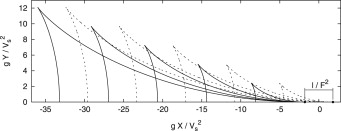
\includegraphics[width=0.5\textwidth]{chap1/longKel.jpg}
  \bicaption[fig:longintrf]{单体船首尾波系的叠加}
  {位于单体船首尾区域的两兴波点产生的开尔文波系的叠加}{Fig}
  {Superposition of two Kelvin wave patterns with origins (marked as dots)
located at the bow and the stern of a monohull ship}
\end{figure}

\begin{figure}[htp]
  \centering
  \captionstyle{\centering}
  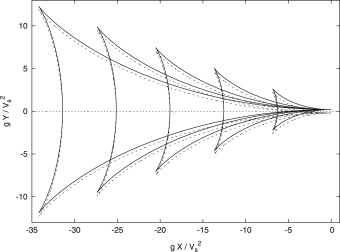
\includegraphics[width=0.5\textwidth]{chap1/latKel.jpg}
  \bicaption[fig:longintrf]{双体船两片体首波系的叠加}
  {位于双体船两片体首部的两兴波点产生的开尔文波系的叠加}{Fig}
  {Superposition of two Kelvin wave patterns with origins (marked as dots)
located at the bows of the twin hulls of a catamaran}
\end{figure}

定义如下弗洛德数
\begin{subequations}\label{eq:Fdef}
  \begin{eqnarray}
    F\equiv V/\sqrt{gL} \label{eq:Fdef-a}\\
    F_s\equiv V/\sqrt{gS}
    \label{eq:Fdef-b}
  \end{eqnarray}
\end{subequations}
\parencite{Noblesse2014Why}证明当$F>F^x$时,单体船首尾兴波的散波成分间的纵向干涉
(longitudinal interference) 会在与航迹成$\psi=\pm\psi^x_{\max}$的射线上产生波高最大
的波。$F^x$与$\psi^x_{\max}$由下式给出
\begin{subequations}\label{eq:psixym}
  \begin{equation}
    \psi^x_{max}\approx\arctan(0.16\ell_e/F^2),\quad F^x\approx 0.59
    \label{eq:psixm}
  \end{equation}
这里,$\ell_e$是位于船首的点源与位于船尾的点汇之间的距离。考虑到首波的波峰总是
出现在船首偏后位置,而尾波的波谷出现船尾靠前位置,工程上常用$\ell_e\approx0.9$
表示这段距离。

类似地,当$F_s>F_s^y$时,双体船两片体首部兴波的散波成分间的横向干涉 
(lateral interference) 会在与航迹成$\psi^y_{\max}$的射线上产生波高最大的波。
$F^y_s$与$\psi^y_{\max}$由下式给出
\begin{equation}
  \psi^y_{\max}\approx\arctan(0.2/F_s),\quad F^y_s\approx 0.37
  \label{eq:psiym}
\end{equation}
\end{subequations}

式\eqref{eq:psixm}与\eqref{eq:psiym}表明,由纵向干涉产生的主要兴波角$\psi^x_{\max}$
以$1/F^2$的形式减小,而由横向干涉产生的主要兴波角$\psi_{\max}^y$则以$1/F_s$的形式
减小。\parencite{Noblesse2014Why}考虑的两点兴波模型 (2-point wavemaker model) 
中的纵向干涉和横向干涉是分布在船体表面的点源间相互干涉的两种基本情况。
两点兴波模型明确揭示了主要兴波角$\psi_{\max}$小于开尔文角$\psi^K$的现象是由于波浪的
相互干涉产生的。其结果为船体兴波的主要兴波角$\psi_{\max}$提供了简单实用的估计,如图 5所示。


\begin{figure}[htp]
  \centering
  \captionstyle{\centering}
  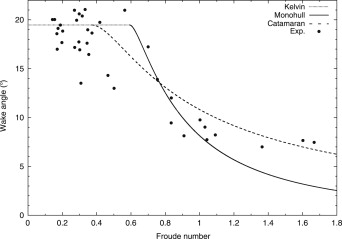
\includegraphics[width=0.5\textwidth]{chap1/longlat.jpg}
  \bicaption[fig:twopwavmkr]{两点兴波模型得出的主要兴波角$\psi_{\max}$的大小}
  {考虑单体船首尾波系以及双体船两片体首波系干涉效应的两点兴波模型预测的
    主要兴波角$\psi_{\max}$的大小}{Fig}
    {Theoretical predictions given by the two-point wavemaker model 
      of interference between the divergent waves created by the bow 
      and the stern of a monohull or between the bows of the twin 
    hulls of a catamaran}
\end{figure}

至此我们可以看到,窄V字形船行波是由高速时散波的干涉效应产生的。
两兴波点的横向或纵向相干干涉会使$\psi=\pm\psi_{\max}$射线上的波浪波高增加,
因此该处的波在观测时更容易受到注意。两点兴波模型作为开尔文压力点兴波理论的扩展,
预测的单体船和双体船的主要兴波角与观测结果基本一致,表明了该理论的正确性。
同时,我们也可以看到散波干涉对波形的影响只在高速时(对单体船而言,$F>0.59$)才明显,而一般的排水型船舶很难达到这一航速,这可能是散波干涉长期被忽视的原因之一。

虽然波浪干涉效应在以往的研究中\supercite{Mei1991Note,Zhu2008Resonant,Fang2011Kelvin,Rabaud2013Ship,Darmon2014Kelvin}
被忽视,它存在于各种各样的波动中,如光、无线电、声波、水波、物质波。
事实上,船周围流场速度由幅值随距离$h\equiv\sqrt{x^2+y^2}$以$1/\sqrt{h}$衰减的
波动部分(wave component)和以$1/(x^2+y^2+z^2)^{3/2}$衰减的局部流动部分
(local flow component)组成。在距离船相对较小的距离外,
船产生的流动主要由向外自由传播的波浪线性叠加而成。
因此波浪之间的干涉作用是决定船行波波形的最主要的物理机理。

由于两点兴波模型\supercite{Noblesse2014Why}将船体简化成两个兴波点,
模型预测的主要兴波角$\psi_{\max}$不可能非常精确。
而\parencite{Darmon2014Kelvin}虽然通过理论证明和数值计算给出了主要兴波角的解析式,
但结果基于压力的高斯分布形式。正如前面提到的,船体表面的压力分布一般在首尾驻点附近
存在最大压力区,因此这种压力分布的兴波很难代表船体的兴波(除非对于滑行艇)。
此外,\parencite{Darmon2014Kelvin}的解析式是在高弗洛德数 ($F>2$) 情况下得出的
渐近结果,即使高速船也很难达到,因此工程实用性不强。

\subsection{波形的数值计算}
考虑在线性势流理论的框架下,船长为$L$的船以航速$V$在无限深广静水中直线航行时所产生
的远场波。观察流动的参考系是固结在船体上与船体一起运动的伽利略参考系$\mathbf{X}=(X,Y,Z)$,
因而流动从参考系观察是定常的。流场的速度可以看作均匀来流的速度$(-V,0,0)$与扰动速度
$(\Phi_X,\Phi_Y,\Phi_Z)$的叠加,其中$\Phi(\mathbf{X})$是扰动速度势。将未扰动的自由
面定义为$Z=0$且$Z$轴竖直向上,$X$轴与船的航向一致且指向船首。用船长$L$以及航速
$V$定义无因次化的坐标系$\mathbf{x}\equiv\mathbf{X}/L$、扰动速度势$\phi=\Phi/VL$、
以及速度场$\nabla_\mathbf{x}\phi\equiv(\phi_x,\phi_y,\phi_z)\equiv(\Phi_X,\Phi_Y,\Phi_Z)/V$。

在线性势流理论的框架内,船体周围的流场可以表示成分布于船体表面的奇点(点源与点汇)
诱导的流场。这些奇点与满足线性自由面条件的基本解(格林函数)相联系。这些被称为自由面
格林函数的基本解已经被广泛研究\supercite{Noblesse1981Alternative}。
分布于船体表面的点源其密度可以由船体曲面形状显式表出,如Hogner近似\supercite{Hogner1932Hydromech}或者与之类似的细长船体理论\supercite{Noblesse1983slender}
(slender-ship approximation),也可通过Neumann-Kelvin (NK) 理论\supercite{Brard1972representation,Gueval1974distribution}
或与之相关的Neumann-Michell (NM) 理论\supercite{Noblesse2013Neumann}
通过数值计算确定。Hogner近似或细长船体理论分别是NM理论或NK理论的近似解
\supercite{Noblesse1983slender,Noblesse2013Neumann}。
细长船体理论与薄船理论\supercite{Michell1898wave}(thin ship theory)密切相关,
可以看作是薄船理论的延伸。

Hogner近似虽然没有NM理论精确,但是既简单又实用。特别地,基于Hogner近似预报的多艘船
在范围广泛的弗洛德数$F$区间内的升沉、纵摇、阻力和自由面升高与实验结果以及NM理论的
预报结果一致\supercite{Noblesse2013Neumann,Huang2013Numerical}。
Hogner近似将船体周围的流场显式表达成弗洛德数$F$和船体曲面形状的函数,
因而比NM理论简单得多。
在Hogner理论中,分布于船体表面的点源密度等于曲面法向量$\mathbf{n}\equiv(n^x,n^y,n^z)$的$x$分量$n^x$。


尽管薄船理论\supercite{Michell1898wave}早在1898年就被提出并被用于估算兴波阻力,
波形的计算直到一个世纪后才出现。理论上薄船理论可直接用于波形的数值模拟,
但由于每个场点的波高都需要计算一个三重积分,所以在计算机产生之前波形的模拟未能实现。
事实上,由于没有Michell积分的计算程序,薄船理论在船舶工程和水动力学实验室并未受到
大量应用。随着计算机科学的进步,现在科学家已经能够通过数值模拟获得复杂的船行波图像。
Ernie Tuck对波形计算做过深入研究。他基于薄船理论编写了快速计算波形的程序,
对于一艘驱逐舰的计算结果与试验波形吻合良好,且并不比考虑
非线性和粘性效应的程序差\supercite{Tuck1971ship,Tuck2001Ship}。
图\ref{fig:tuckwavpat}是基于薄船理论预报的一艘驱逐舰在30节航速下的波形。
值得一提的是,Tuck很早就注意到利用多体船片体之间的波浪干涉可合理布置片体位置
减小兴波阻力,并对纵向错开和不错开的双体、三体和四体船的片体位置的最有布置进行了
研究\supercite{Tuck1998Optimum}。

\begin{figure}[htp]
  \centering
  \captionstyle{\centering}
  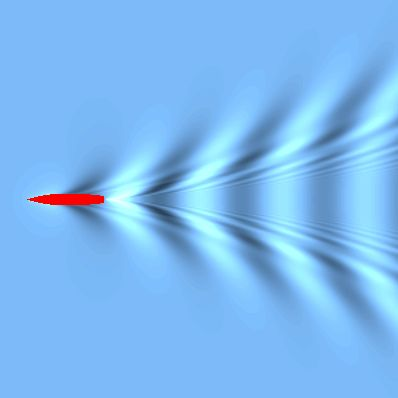
\includegraphics[width=0.5\textwidth]{chap1/eot.jpg}
  \bicaption[fig:tuckwavpat]{薄船理论预报的波形}
  {薄船理论预报的一艘驱逐舰在30节航速时的波形\supercite{Tuck2001Ship}}{Fig}
    {Wave pattern of a destroyer hull at 30 knots predicted via thin-ship theory}
\end{figure}

在线性势流理论的框架里,船行波可表示成一系列正弦波$E=e^{\mathbf{i}h\varphi}$
的线性叠加,这些波的无因次波长在$0\le\lambda\le2\pi F^2$范围内。
因此,线性势流理论得出的船行波中包含了波长非常短的短波,而这些短波在现实中由于受到
表面张力和粘性的影响不可能存在。通过线性外插法,\parencite{Noblesse2013Evaluation}
过滤掉了短波。数值计算结果与试验吻合较好,证明了过滤短波在获得合理波形中的重要性。
另一方面,正弦波的振荡频率随距离$h$的增加而增加,因此对于远场$H\gg L$或低弗洛德数$F$
的情况,波的傅里叶积分中被积函数是快速振荡的。如果要通过直接积分获得较精确的结果,
需要布置大量的积分点,这显然是不现实的。基于开尔文的驻相法可以简化傅里叶积分,
获得$h\gg 1$时的渐近表达式。但表达式只在开尔文楔内$-\psi^K<\psi<\psi^K$有效,
在$\psi=\pm\psi^K$是发散的。\parencite{Chester1957extension}通过变量代换法获得了
傅里叶积分 (wave integral) 在包括波峰尖顶角 (cusp angle) 的区域都正则的
一致渐近展开式 (uniform asymptotic expansion)。然而展开式形式复杂,
其中包括艾利函数 (Airy Function) 和它的一阶导数,不适合实际使用。
\parencite{Zhang2015Stationary}提出了一种计算自由面任意点波高的实用方法。
这种方法受开尔文的驻相法启发,通过修改振荡的被积函数,消除振荡特性,但不改变
被积函数中对积分有主要贡献的部分。这种方法可用较少的积分点获得较精确的积分值。

由于用计算流体力学 (Computational Fluid Dynamics, CFD) 方法预报波型需要
大量计算资源和计算时间,因此用CFD进行窄V字型船行波的参数化研究并不可行。
\parencite{Wang2015Numerical}用CFD方法模拟了高速船的波形,单个算例的网格量
约为800万,用IB网络连接的英特尔至强处理器32E5-2670计算大约需要300小时。


\subsection{小结}

需要指出的是,造成窄V字形船尾迹的原因很多,非线性、船舶摇荡运动、环境波浪、风,
以及有限水深\supercite{Brown1989Observations,Mei1991Note,Zhu2008Resonant,
Shugan2006Kelvin,Fang2011Kelvin}都会显著地影响Kelvin波系。
此外雷达成像也会影响SAR图像上的窄V字形船尾迹,
Kelvin波系中靠近船中心线附近的短波的布拉格散射 (Bragg scatterin) 
会在明显小于Kelvin角的范围内产生强雷达反射波,从而在SAR图像上产生明亮的线
\supercite{Reed2002Ship,Milgram1988theory}。
尽管目前对于窄V字形船尾迹由稳定的Kelvin波系还是相关的非定常运动造成的还存在争议,
但Kelvin波系是产生窄V字形船尾迹的主要来源,而基于优势波 (dominant waves) 
---船首波和船尾波---干涉效应的两点兴波模型\supercite{Noblesse2014Why}是解释
窄V字形船尾迹最简单且非常合理的模型。

由于两点兴波模型\supercite{Noblesse2014Why}将船体简化成两个兴波点,式
\eqref{eq:psixm}与\eqref{eq:psiym}对主要兴波角$\psi_{\max}$的估计不能预期是非常准确
的。而\parencite{Darmon2014Kelvin}虽然通过理论证明和数值计算给出了主要兴波角
$\psi_{\max}$的解析式,但结果基于压力的高斯分布形式。正如前面提到的,
船体表面的压力分布一般在首尾驻点附近存在最大压力区,
因此这种压力分布的兴波很难代表船体的兴波(除非对于滑行艇)。
此外,\parencite{Darmon2014Kelvin}的解析式是在高弗洛德数 ($F>2$) 情况下得出的
渐近结果,即使高速船也很难达到,因此实用性不强。

实际单体船的兴波比两点兴波模型要复杂得多。
在线性势流理论的框架看来,单体船的兴波是由连续分布于船体表面的点源的兴波叠加而成。
因此波浪干涉效应对单体船的影响既包括纵向干涉效应又包括横向干涉效应的影响。
双体船的波浪干涉还包括两片体点源兴波之间的干涉。
因此考虑整个船体产生的波浪之间的相互干涉效应对Kelvin波系的影响
比两点兴波模型更加接近实际情况。

对窄V字形船尾迹的研究,在线性势流理论的范围内还存在下列重要问题。
一个值得研究的问题是,船体形状的变化对主要兴波角的影响多大?
如果影响不大,我们就可以忽略船体形状对主要兴波角的影响,
并给出适用于一般船的主要兴波角的解析式。
有了该解析式后,我们无需计算就可以预报单体船或双体船在某航速下的主要兴波角,
这在工程上是非常有用的。
要分析船体形状变化对主要兴波角的影响,可以考虑主要船型参数的变化对主要兴波角的影响。
对于单体船而言,主要船型参数有长宽比、长度吃水比、型宽吃水比、半进流角,
对于双体船而言,还需考虑片体间距。
为了得到一般船主要兴波角的解析式,需要进行参数化研究。
对于单体船需要研究包括四个主要船型参数和Froude数共五个参数,
对于双体船,还需研究片体间距的影响。因此需要计算的算例的数量是很大的。这
就对计算程序的效率提出了要求。如果用CFD程序计算(即数值求解NS方程),
虽然可以得到自由面的波形,但是耗时巨大。而且这里要研究的主要是远场波形,
因此需要很大的计算域,即使不考虑CFD方法存在数值耗散等问题,
仅仅考虑计算量和计算资源的问题,也令人望而生畏。
因此用CFD方法预报远场波形不可行。我们需要采用一种快速计算远场波形的算法。

另一个有趣的问题是,两点兴波模型预测的主要兴波角精确程度如何?
在有了一般单体船或双体船主要兴波角的解析式后,我们可以将其与两点兴波模型得出的结果
---式\eqref{eq:psixm}和\eqref{eq:psiym}---进行比较,分析两点兴波模型的准确性。
我们还可以分析横向干涉与纵向干涉对单体船和双体船主要兴波角的影响哪个占主导。
将单体船的兴波简化为首尾两点的兴波能考虑首尾波系的干涉,
但是无法反映左右舷侧的点源兴波的干涉。从前面的分析可知,两点纵向干涉产生的
主要兴波角随弗洛德数$F$以$1/F^2$的形式衰减,而两点横向干涉使主要兴波角
随弗洛德数$F_s$以$1/F_s$的形式衰减。因此随着航速$V$的增大,
横向干涉对单体船主要兴波角的影响应该会逐渐占据主导。
我们还不知道从纵向干涉主导到横向干涉主导之间是如何转变的?
是逐渐转变的还是骤变的?转变发生在什么时候?对双体船而言,也有类似的问题。


\section{论文主要内容与章节安排}
\label{sec:plan}



